%-----------------------------------------------------------------------------%
\chapter{\babEmpat}
%-----------------------------------------------------------------------------%
Bab ini menjelaskan secara detail proses implementasi dari pengolahan data, proses \textit{pattern extraction} dan \textit{matching}, pembobotan dan \textit{ranking} baik \textit{pattern} maupun \textit{pair}.

\begin{figure}
    \centering
    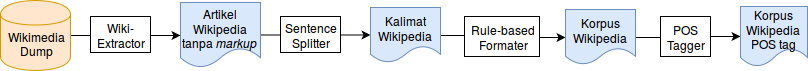
\includegraphics[width=\linewidth]{pics/Pic02-PreProcessingWikipedia}
    \caption{Pre-processing Data Wikipedia}
    \label{fig:preproses-wiki}
\end{figure}
%-----------------------------------------------------------------------------%
\section{Pembentukan Korpus Kalimat Wikipedia}
%-----------------------------------------------------------------------------%
Data hasi Wikipedia Dump diformat secara otomatis menggunakan \textit{tools} WikiExtractor. WikiExtractor adalah program berbasis Python yang dibuat oleh Giuseppe Attardi dan Antonio Fuschetto. Menggunakan \textit{tools} ini, didapatkan data yang sudah tidak mengikuti format MediaWiki Markup Language. Program ini dapat diunduh dari Github dan dijalankan menggunakan perintah berikut. 
\begin{lstlisting}[language=bash]
  $ WikiExtractor.py xml-dump-file -o output-file
\end{lstlisting}
Jika tidak memberi spesifikasi opsi apapun, artikel yang dihasilkan membersihkan seluruh markup language dan hanya menyimpan isi artikel tanpa disertakan informasi seperti kategori, riwayat, dan versi artikel.

%-----------------------------------------------------------------------------%
\subsection{Sentence Splitting}
%-----------------------------------------------------------------------------%
Korpus yang dihasilkan menghasilkan baris-baris yang merepresentasikan suatu paragraf dalam artikel Wikipedia. Pada penelitian kali ini, ingin dilihat relasi \textit{hypernym-hyponym} antar dua kata pada kalimat yang sama. Untuk itu, perlu dilakukan proses \textit{sentence splitting} yang dapat mengidentifikasi suatu kalimat dalam paragraf. Hasil dari proses tersebut adalah dokumen yang terdiri dari baris-baris yang merepresentasikan satu kalimat. 

Proses ini dilakukan dengan menggunakan \textit{script} yang telah dibuat sebelumnya oleh Ken Nabila Setya dari Fasilkom UI, Indonesia. Ditambah pula satu \textit{script} yang dapat secara otomatis melakukan \textit{splitting} untuk seluruh dokumen. Berikut adalah contoh sebuah paragraf dalam artikel Wikipedia yang telah dibersihkan menggunakan WikiExtractor.
\begin{center}
\begin{tabular}{ | m{32em} | } 
\hline
Charles Anthony Johnson (3 Juni 1829 - 17 Mei 1917), kemudian dikenal sebagai Charles Brooke memerintah Sarawak sebagai Raja Putih kedua dari 3 Agustus 1868 hingga meninggal dunia. Dia menggantikan pamannya, James Brooke sebagai raja. \\
\hline 
\end{tabular}
\end{center}

\noindent Setelah melalui proses \textit{sentence splitter}, berikut adalah hasilnya.
\begin{center}
\begin{tabular}{ | m{32em} | } 
\hline
Charles Anthony Johnson (3 Juni 1829 - 17 Mei 1917), kemudian dikenal sebagai Charles Brooke memerintah Sarawak sebagai Raja Putih kedua dari 3 Agustus 1868 hingga meninggal dunia. \\
\hline 
 Dia menggantikan pamannya, James Brooke sebagai raja. \\
\hline
\end{tabular}
\end{center}

%-----------------------------------------------------------------------------%
\subsection{Rule Based Formatter}
%-----------------------------------------------------------------------------%
Dari korpus yang berisi kalimat Wikipedia, diberikan beberapa aturan tambahan untuk membuat korpus sesuai format yang diinginkan. Penambahan aturan juga untuk mengurangi ambiguitas dan bentuk usaha generalisasi \textit{pattern}. Berikut adalah beberapa aturan tambahan untuk \textit{pre-processing} korpus Wikipedia.
\begin{enumerate}
  \item Menghilangkan frase yang berada di dalam tanda kurung. \\
  Frase yang terletak di dalam tanda kurung dapat dianggap sebagai penjelas kata atau frasa sebelumnya. Proses ini merupakan salah satu upaya generalisasi \textit{pattern}.
  \item Memisahkan simbol-simbol yang berhimpit pada awal dan akhir kata. \\
  Beberapa token yang dipisahkan oleh spasi dalam kalimat merupakan kata yang berhimpit dengan tanda baca. Untuk mempermudah proses selanjutnya yaitu \textit{sentence tagging}, dilakukan \textit{pre-processing} tambahan yaitu memisahkan simbol-simbol \textit{non-alphanumerical}.
  \item Memberi penanda awal kalimat dengan '<start>'' dan akhir kalimat dengan '<end>'. \\
  Pemberian simbol awal dan akhir kalimat memperjelas isi kalimat dan juga menunjang proses \textit{pattern extraction} dan \textit{pattern matching}.
\end{enumerate}

\noindent Dari contoh kalimat di atas, setelah melalui proses \textit{formatting} yang didefinisikan menghasilkan kalimat berikut.
\begin{center}
\begin{tabular}{ | m{32em} | } 
\hline
<start> Charles Anthony Johnson , kemudian dikenal sebagai Charles Brooke memerintah Sarawak sebagai Raja Putih kedua dari 3 Agustus 1868 hingga meninggal dunia . <end> \\
\hline 
<start> Dia menggantikan pamannya , James Brooke sebagai raja . <end> \\
\hline
\end{tabular}
\end{center}


%-----------------------------------------------------------------------------%
\section{POS Tagging Kalimat Wikipedia}
%-----------------------------------------------------------------------------%
Proses \textit{part-of-speech tagging} dilakukan pada korpus Wikipedia yang telah berbentuk kalimat dengan format yang didefinisikan. Pada penelitian ini, kelas kata yang menjadi pengamatan adalah \textit{noun} (NN) dan \textit{proper noun} (NNP), sehingga proses \textit{pos tagging} digunakan untuk identifikasi kata-kata tersebut. Proses \textit{pos tagging} menggunakan \textit{tools} Stanford POS Tagger, dengan model yang digunakan merupakan hasil penelitian sebelumnya menggunakan Bahasa Indonesia.  Setelah selesai melalui proses \textit{tagging}, dilakukan penyesuaian agar format korpus lebih rapi dan terstruktur. 

Berikut adalah contoh kalimat yang sudah melalui tahap \textit{pos tagging}. Korpus ini digunakan untuk proses \textit{pattern matching}.
\begin{center}
\begin{tabular}{ | m{32em} | } 
\hline
<start>\_X Charles\_NNP Anthony\_NNP Johnson\_NNP ,\_Z kemudian\_CC dikenal\_VB sebagai\_IN Charles\_NNP Brooke\_NNP memerintah\_VB Sarawak\_NNP sebagai\_IN Raja\_NNP Putih\_NNP kedua\_CD dari\_IN 3\_CD Agustus\_NNP 1868\_CD hingga\_IN meninggal\_VB dunia\_NN .\_Z <end>\_X \\ 
\hline
\end{tabular}
\end{center}


\begin{figure}
    \centering
    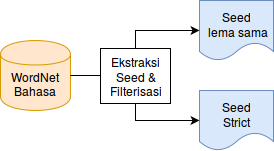
\includegraphics[width=\linewidth]{pics/Pic02-SeedBuilder}
    \caption{Proses Pembentukan \textit{Seed}}
    \label{fig:seed-builder}
\end{figure}
%-----------------------------------------------------------------------------%
\section{Seed Builder}
%-----------------------------------------------------------------------------%
Proses pengumpulan \textit{seed} dibantu dengan \textit{resource} yang dimiliki WordNet Bahasa menggunakan \textit{tools} nltk. Proses pengumpulan diawali dengan mengambil seluruh lema Bahasa Indonesia yang dimiliki oleh korpus nltk. Setelah itu, ambil seluruh \textit{synset} yang mengandung lemma tersebut. Dari setiap \textit{synset}, ambil relasi \textit{hypernym}-nya. Dari setiap \textit{synset} relasi, ambil lema Bahasa Indonesianya. Dilakukan pula filterisasi \textit{synset} ataupun lema untuk mengurangi ambiguitas. Untuk setiap \textit{synset} maupun lema yang diambil pada setiap tahapan, hanya boleh berasal dari kelas kata kerja (\textit{noun}). Setelah didapatkan, bentuk ke dalam pasangan \textit{tuple} 1-1 $(kata\_hyponym,kata\_hypernym)$.

%-----------------------------------------------------------------------------%
\subsection{Filterisasi Seed}
%-----------------------------------------------------------------------------%
Filterisasi dilakukan dengan tujuan mengurangi ambiguitas, namun tetap berusaha mendapatkan \textit{seed} sebanyak mungkin. Filterasisasi juga dilakukan untuk mendapatkan \textit{seed} awal yang diyakini benar dan berkualitas. Salah satu bagian terpenting proses ini adalah memasangkan hanya lema yang merupakan \textit{noun} ke lema yang juga adalah \textit{noun}. Jika kemungkinan lema tersebut tergolong ke dalam kelas kata bukan \textit{noun}, lema tidak diikutsertakan sebagai \textit{seed} awal.

Tantangan dalam proses ini adalah banyak ditemukan kasus dimana satu lema dikandung oleh lebih dari satu \textit{synset} atau satu \textit{synset} memiliki lebih dari satu \textit{synset hypernym}. Ambiguitas dalam kasus tersebut dapat mengurangi kualitas \textit{seed} yang dihasilkan. Mengatahui hal tersebut, dibuatlah dua pendekatan berbeda untuk proses filterisasi \textit{seed}.

Pendekatan pertama adalah tetap mengambil lemma yang sama pada \textit{synset hypernym} yang berbeda. Hal ini dilatarbelakangi adanya lema yang berasal dari \textit{synset} berbeda namun memiliki lema \textit{hypernym} yang sama. Pada contoh (i), satu lema yang sama dimiliki oleh dua \textit{synset} yang berbeda namun kedua \textit{synset} tersebut memiliki \textit{synset hypernym} yang sama. Pada contoh (ii), satu lema berasal dari dua \textit{synset} yang berbeda dan dua \textit{synset hypernym} berbeda, namun ada lema yang sama yaitu 'laluan'.

Pendekatan lainnya adalah dengan metode filterisasi yang paling ketat. Jika satu lema memiliki lebih dari satu \textit{synset hypernym}, maka lema tersebut dianggap ambigu dan langsung tidak diikutsertakan ke dalam \textit{seed} awal. Berdasarkan tabel contoh lema, \textit{synset}, dan \textit{hypernym}-nya, hanya contoh (i) yang diterima sebagai \textit{seed} karena \textit{synset hypernym} untuk lema tersebut sama. Sementara (ii) ditolak karena \textit{synset hypernym} berbeda.

\begin{center}
\begin{tabular}{ |c|m{30em}| } 
\hline
\multirow{2}{*}{i.} & ('paruh', Synset('beak.n.02')) => (['bibir', 'kuala', 'muara'], [Synset('mouth.n.02')])
('paruh', Synset('beak.n.01')) => (['bibir', 'kuala', 'muara'], [Synset('mouth.n.02')]) \\ 
& ('paruh', Synset('beak.n.01')) => (['bibir', 'kuala', 'muara'], [Synset('mouth.n.02')]) \\ 
\hline
\multirow{2}{*}{ii.} & ('pintu\_masuk', Synset('entrance.n.01')) => (['akses', 'capaian', 'laluan'], [Synset('access.n.03')]) \\ 
& ('pintu\_masuk', Synset('orifice.n.01')) => (['koridor', 'laluan', 'lorong'], [Synset('passage.n.07')]) \\ 
\hline
\end{tabular}
\end{center}

%-----------------------------------------------------------------------------%
\subsection{Kelemahan Seed yang Dihasilkan}
%-----------------------------------------------------------------------------%
Walau sudah dilakukan proses filterisasi untuk meningkatkan kualitas \textit{seed}, masih ada hambatan yang belum bisa diatasi dalam penelitian ini. Beberapa kelemahan dari \textit{seed} awal yang dihasilkan, antara lain:
\begin{itemize}
  \item \textit{Seed} yang mengandung kata bukan Bahasa Indonesia. Korpus yang ingin dibuat berdomain Bahasa Indonesia, namun \textit{seed} yang dihasilkan mengandung Bahasa Melayu atau Bahasa Indonesia lama. Beberapa kata bukan Bahasa Indonesia yang dihasilkan adalah 'had', 'bonjol', dan 'cecok'.
  \item Kesalahan semantik \textit{synset} dan lema Bahasa Indonesia. Beberapa \textit{synset} nltk memiliki lema Bahasa Indonesia yang kurang sesuai jika dilihat secara semantik. Sebagai contoh Synset('scholar.n.01')$ dengan lemma Bahasa Indonesia ${'buku\_harian', 'pelajar'}. Dalam Bahasa Indonesia, 'buku\_harian' memiliki makna yang berbeda dengan 'pelajar'.
  \item Kesalahan lema Bahasa Indonesia untuk suatu \textit{synset} menyebabkan dihasilkannya \textit{seed} yang jika dievaluasi kualitatif oleh manusia dirasa kurang tepat. Contoh \textit{seed} yang tidak baik adalah dari pemetaan $('sejarawan', Synset('historian.n.01')) => (['buku\_harian', 'pelajar'], [Synset('scholar.n.01')])$ dihasilkan \textit{seed} $(sejarawan,buku harian)$ dan $(sejarawan,pelajar)$. \textit{Seed} $(sejarawan,buku harian)$ adalah salah.
\end{itemize}


\begin{figure}
    \centering
    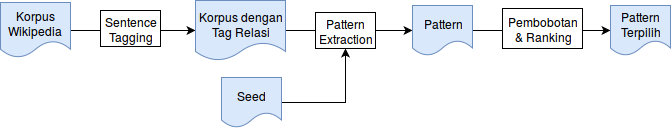
\includegraphics[width=\linewidth]{pics/Pic03-PatternExtraction}
    \caption{Proses Pembentukan \textit{Pattern}}
    \label{fig:pattern-extraction}
\end{figure}
%-----------------------------------------------------------------------------%
\section{Sentence Tagging}
%-----------------------------------------------------------------------------%
Setelah memperoleh pasangan kata relasi Bahasa Indonesia, perlu dilakukan \textit{tagging} pasangan kata tersebut ke kalimat-kalimat dalam korpus Wikipedia. Data yang digunakan untuk proses ini adalah korpus Wikipedia tanpa \textit{pos tag}. Beberapa tahapan dilakukan pada proses \textit{tagging sentence} dengan pasangan kata relasi adalah sebagai berikut.
\begin{enumerate}
  \item Dibaca seluruh pasangan kata relasi \textit{hyponym-hypernym}.
  \item Untuk setiap kalimat pada korpus Wikipedia, di cek apakah kalimat tersebut mengandung pasangan kata relasi.
  \item Pengecekan dilakukan secara berulang untuk seluruh pasangan kata relasi karena terdapat kemungkinan satu kalimat mengandung lebih dari satu pasang kata relasi.
  \item Kata-kata yang merupakan bagian dari pasangan kata relasi kemudian di-\textit{tag} sesuai relasinya dan disimpan ke dalam korpus berisi kalimat dengan \textit{tag} \textit{hyponym} dan \textit{hypernym}.
\end{enumerate}

Pada penelitian ini, satu kalimat yang telah di-\textit{tag} hanya mengandung tepat satu pasangan kata relasi. Untuk kasus khusus dimana suatu pasangan kata relasi terdiri dari satu kata yang merupakan sub kata pasangannya, maka pasangan kata tersebut tidak diikutsertakan untuk menghindari ambiguitas. Contoh pasangan kata yang tidak diikutsertakan adalah $(ikan\,\,gurame;ikan)$, kata 'ikan' terkandung dalam kedua kata relasi. 

Berikut adalah contoh kalimat yang terbentuk dari proses \textit{sentence tagging}. Diberikan pasangan kata relasi \textit{hyponym-hypernym} $(fermion;partikel)$ dan $(boson;partikel)$ serta kalimat  '<start> seluruh partikel dasar adalah boson atau fermion . <end>'. Hasil proses \textit{sentence tagging} adalah sebagai berikut.
\begin{center}
\begin{tabular}{ | m{32em} | } 
\hline
<start> seluruh <hypernym>partikel<hypernym> dasar adalah boson atau <hyponym>fermion<hyponym> . <end> \\ 
\hline
\hline
<start> seluruh <hypernym>partikel<hypernym> dasar adalah <hyponym>boson<hyponym> atau fermion . <end> \\ 
\hline
\end{tabular}
\end{center}


%-----------------------------------------------------------------------------%
\section{Pattern Extraction}
%-----------------------------------------------------------------------------%
Setelah mendapatkan kalimat-kalimat yang telah di-tag dengan kata relasi, ingin dicari pattern yang dapat digunakan untuk menambah jumlah relasi kata. Pembuatan pattern menggunakan algoritma dasar Standard Trie dengan beberapa modifikasi. Proses ini diimplementasi secara mandiri menggunakan program Java dengan mengikuti algoritma pembuatan Trie sederhana.

Suatu node merepresentasikan kata dalam kalimat dan dari satu kalimat terbentuk sebuah cabang dalam tree. Node menyimpan beberapa informasi seperti nama node, parent, childs, dan informasi identitas tambaha seperti apakah node tersebut merupakan relasi dan apakah node tersebut merupakan leaf. Untuk kata yang merupakan kata relasi, node menyimpan informasi jenis relasi beserta list dari kata yang merupakan bagian dari relasi tersebut. Sebagai contoh dua kalimat sebagai berikut.
\begin{center}
\begin{tabular}{ | m{32em} | } 
\hline
<start> <hyponym>singa<hyponym> adalah <hypernym>kucing<hypernym> yang berukuran besar <end> \\ 
\hline
\hline
<start> <hyponym>serigala<hyponym> adalah <hypernym>anjing<hypernym> yang tinggal di hutan <end>\\ 
\hline
\end{tabular}
\end{center}

Akan menghasilkan Pattern Tree sebagai berikut. Angka setelah kata adalah bobot suatu node.
% TODO: insert coontoh pattern tree

%-----------------------------------------------------------------------------%
\subsection{Informasi dalam Pattern}
%-----------------------------------------------------------------------------%
Beberapa informasi yang disimpan dalam suatu pattern adalah sequence kata, jumlah kemunculan dalam korpus,  seed unik yang membentuk pattern tersebut, dan kalimat unik yang membentuk pattern tersebut. Informasi-informasi tersebut nantinya digunakan untuk memberi bobot pattern dan melakukan sorting pemilihan pattern terbaik.

%-----------------------------------------------------------------------------%
\subsection{Pattern Tree}
%-----------------------------------------------------------------------------%
Pattern Tree adalah sebuah tree yang menyimpan seluruh pattern yang dihasilkan dari korpus. Dalam pembuatan Pattern Tree, tidak perlu menyimpan seluruh kata dalam kalimat. Hanya sequence kata tertentu saja yang dianggap dapat menghasilkan pattern yang baik untuk diikutsertakan. Maka dari itu, perlu diambil sequence kata dalam kalimat yang digunakan sebagai pattern. Terdapat tiga pendekatan dalam proses ini, diantaranya:
\begin{enumerate}
  \item Hanya memperhatikan kata yang berada diantara kata relasi. Pada kasus ini, hanya ingin dilihat kata-kata yang berada diantara kata yang merupakan hypernym-hyponym atau hyponym-hypernym. Kata-kata diantara dua relasi dapat dianggap paling dekat jika ingin mencari pattern relasi tersebut. \\Pada contoh diatas, sequence kata yang dihasilkan adalah '<hyponym>singa<hyponym> adalah <hypernym>kucing<hypernym>'
  \item Mengikutsertakan n kata sebelum kata relasi pertama. Beberapa kata sebelum kata relasi, dapat memberikan informasi untuk yang dapat meningkatkan kualitas pattern yang dihasilkan.\\
  Pada contoh diatas dengan (n=1), sequence kata yang dihasilkan adalah '<start> <hyponym>singa<hyponym> adalah <hypernym>kucing<hypernym>'
  \item Mengikutsertakan n kata setelah kata relasi terakhir. Tipe ini sama dengan sebelumnya, namun dilihat pengaruh kata-kata yang mengikuti kata relasi. \\
  Pada contoh diatas dengan (n=1), sequence kata yang dihasilkan adalah '<hyponym>singa<hyponym> adalah <hypernym>kucing<hypernym> yang'
\end{enumerate}

%-----------------------------------------------------------------------------%
\subsection{Vektor Pattern}
%-----------------------------------------------------------------------------%
Suatu pattern dapat direpresentasikan menjadi vektor berdasarkan nilai-nilai yang dimilikinya. Vektor ini dapat dimanfaatkan untuk menentukan pattern yang baik (pembobotan). Fitur utama pada vektor pattern diambil dari informasi yang disimpan oleh suatu pattern, yaitu total kemunculan pattern, jumlah seed unik, dan jumlah kalimat unik yang membentuk pattern tersebut. Fitur lain adalah hasil kombinasi perbandingan antar nilai utama. Fitur tambahannya adalah nilai perbandingan antara jumlah seed unik dibagi jumlah kalimat unik, nilai perbandingan antara jumlah seed untuk dibagi total kemunculan, dan nilai perbandingan antara jumlah kalimat unik dibagi total kemunculan.

%-----------------------------------------------------------------------------%
\subsection{Validasi dan Filterisasi Pattern}
%-----------------------------------------------------------------------------%
Setelah terbentuk Pattern Tree, perlu di-list seluruh pattern yang dihasilkan. Untuk mengurangi pattern yang kurang baik dihasilkan, perlu dilakukan proses validasi. Proses ini sama seperti proses filtering yang dilakukan pada tahap pengumpulan seed. Beberapa aturan yang harus dipenuhi agar suatu pattern dianggap valid adalah sebagai berikut.
\begin{itemize}
  \item Harus ada minimal satu kata diantara dua kata relasi. Banyak kasus dimana dua kata relasi hanya dipisahkan oleh spasi. Pattern yang hanya mengandung spasi tidak memberikan informasi apapun karena simbol spasi dalam Bahas Indonesia pasti digunakan sebagai pemisah antar kata. Sebagai contoh kalimat hasil tagging '<start> semua jenis <hypernym>ular<hypernym> <hyponym>beludak<hyponym> memiliki taring yang panjang <end>'
  \item Sebuah pattern harus memenuhi nilai threshold yang didefinisikan. Nilai perbandingan antara jumlah seed unik dibagi jumlah kalimat unik lebih dari 0.5. Nilai perbandingan antara jumlah seed unik dibagi total kemunculan lebih dari 0.2. Nilai perbandingan antara jumlah kalimat unik dibagi total kemunculan harus lebih dari 0.7. Ketiga nilai threshold tersebut didefinisikan sendiri berdasarkan pengamatan nilai pada vektor pattern.
\end{itemize}

%-----------------------------------------------------------------------------%
\subsection{Pembentukan Pattern Unik}
%-----------------------------------------------------------------------------%
Pattern yang dihasilkan dari tahap ini harus unik sehingga tidak terjadi ambiguitas jika hendak digunakan. Pada masa awal pengembangan, masalah yang muncul pada pattern yang dihasilkan adalah adanya pattern yang posisi penempatan hypernym-hyponym-nya saling berkebalikan. Sebagai contoh beberapa pattern ambigu yang dihasilkan seperti (i) <hyponym> adalah <hypernym>, (ii) <hypernym> adalah <hyponym>, (iii) <hypernym> dan <hyponym>, dan (iv) <hyponym> dan <hypernym>. Padahal, bagian hypernym-hyponym tersebut nantinya digantikan dengan kata kemunculannya cocok dengan pattern yang diberikan. Jika pattern dibiarkan begitu saja, banyak dihasilkan seed yang salah.

Strategi yang dilakukan untuk masalah ambiguitas antar pattern adalah membangun suatu arsitektur yang dapat mengidentifikasi dan menyelesaikannya. Tahapan pembangunan pattern unik adalah sebagai berikut.
\begin{enumerate}
  \item Dicari pattern dengan pendekatan hanya memperhatikan kata-kata diantara relasi.
  \item Pattern yang dihasilkan dievaluasi satu dengan yang lain. Jika terdapat pattern yang saling terbalik, pattern yang bersangkutan dikeluarkan dari list dan disimpan untuk dievaluasi ulang.
  \item Proses evaluasi ulang dilakukan menggunakan pendekatan pembuatan pattern lainnya yaitu, memperhatikan n kata sebelum atau sesudah kemunculan relasi.
  \item Hasil kedua pendekatan digabung dan dicek apakah pattern tersebut dibutuhkan. Suatu pattern hasil evaluasi ulang dinyatakan dibutuhkan jika substring dari pattern tersebut tergolong dalam list pattern yang membutuhkan evaluasi ulang.
  \item Proses evaluasi dilakukan secara berulang dari dengan n yang terus bertambah dari 1 (satu). Pada penelitian ini, nilai n dibatasi hingga 2 (dua).
\end{enumerate}

Setelah melakukan tahapan di atas, tidak ada lagi kasus posisi relasi saling tertukar dari pattern yang dihasilkan. List pattern yang dihasilkan kemudian di-sorting sebelum ditampilkan.

%-----------------------------------------------------------------------------%
\subsection{Pengurutan Pattern}
%-----------------------------------------------------------------------------%
Setelah didapatkan pattern yang sesuai, dilakukan proses pengurutan (sorting) untuk mengetahui pattern mana yang terbaik berdasarkan bobot yang dimiliki. Proses pengurutan dilakukan dengan membandingkan satu pattern dengan yang lain, dengan tahapan sebagai berikut.
\begin{enumerate}
  \item Semakin besar jumlah kalimat unik yang membentuk pattern.
  \item Semakin besar nilai perbandingan antara jumlah seed unik yang membentuk pattern dengan jumlah kalimat unik yang membentuk pattern.
  \item Semakin kecil jumlah token dalam pattern tersebut jika di-parse dengan spasi.
\end{enumerate}

%-----------------------------------------------------------------------------%
\subsection{Kelemahan Pattern yang Dihasilkan}
%-----------------------------------------------------------------------------%
Hasil dari tahap ekstraksi pattern dengan aturan-aturan di atas memberi pattern yang baik untuk relasi kata hyponym-hypernym. Beberapa masalah yang belum dapat diselesaikan seperti menentukan pattern mana yang lebih baik jika satu pattern adalah substring dari pattern yang lain dan generalisasi pattern. Pada penelitian ini, pattern yang diprioritiskan jika hal tersebut terjadi adalah pattern yang memiliki jumlah token terpendek. Namun, hal tersebut belum bisa dikatakan yang terbaik.

Beberapa pattern terlihat kurang baik secara semantik jika dilihat sekilas. Pattern seperti (a).<hypernym> dan <hyponym> (b) <hypernym> atau <hyponym>, kurang cocok jika digunakan dalam Pattern Matching. Hal ini disebabkan kata 'dan' dan 'atau' memuat relasi yang bersifat simetris. Sementara hypernym-hyponym merupakan relasi yang hanya memiliki sifat transitif. Pada penelitian ini, relasi yang  diamati hanya hypenym-hyponym. Ada kemungkinan suatu pattern yang sama dihasilkan dari beberaparelasi yang lain dan mungkin lebih cocok digunakan utnuk relasi lain tersebut. Tidak adanya perbandingan pattern yang dihasilkan oleh relasi lain menjadi salah satu hambatan memilih pattern yang baik.


\begin{figure}
    \centering
    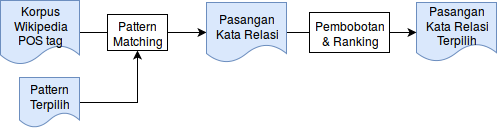
\includegraphics[width=\linewidth]{pics/Pic04-PatternMatching}
    \caption{Proses Pembentukan \textit{Pair}}
    \label{fig:pattern-matching}
\end{figure}
%-----------------------------------------------------------------------------%
\section{Pattern Matching}
%-----------------------------------------------------------------------------%
Pattern yang terbentuk dari proses pattern extraction digunakan untuk menambah jumlah pasangan kata relasi dengan dilakukan proses Pattern Matching terhadap korpus Wikipedia. Proses Pattern Matching menggunakan algoritma Suffix Tree dengan modifikasi. Implementasi dilakukan secara mandiri menggunakan program Java.

Sebuah node merepresentasikan satu kata dalam kalimat. Untuk setiap kalimat, dibentuk sebuah Suffix Tree yang merepresentasikan kalimat tersebut dan selanjutnya dicocokan dengan pattern yang ada. Dibuat pula kelas Pair yang merepresentasikan pasangan kata relasi hypernym-hyponym yang dihasilkan dari proses Pattern Matching. Pair menyimpan informasi seperti total kemunculan seed, total dokumen yang menghasilkan seed, kalimat unik dan pattern unik yang menghasilkan pair.

Tahapan proses Pattern Matching jika diberikan satu kalimat dan satu pattern adalah sebagai berikut.
\begin{enumerate}
  \item Kalimat input dibentuk menjadi suatu Suffix Tree.
  \item Pattern input ditokenisasi ke dalam bentuk list kata. Pattern input pasti mengandung token <hypernym> dan <hyponym>, selanjutnya disebut token relasi.
  \item Jika ditemukan token relasi pada list pattern yang sedang dievaluasi, maka node yang dikunjungi disimpan sementara sesuai dengan relasinya.
  \item Jika token bukan token relasi, maka di evaluasi apakah token sama dengan node yang dikunjungi. Jika sama dievaluasi lebih lanjut jika berbeda maka pattern tidak cocok.
  \item Jika seluruh token pattern telah dievaluasi dan tidak mengalami kegagalan, makan dianggap berhasil dan disimpan dalam bentuk pair.
\end{enumerate}
Setelah dijalankan proses Pattern Matching terhadap korpus Wikipedia dengan pattern hasil ekstraksi, masalah pertama yang ditemukan adalah banyaknya pair yang salah satu atau kedua kata relasinya tidak teramasuk dalam kelas kata noun. Beberapa pair yang salah diantaranya (Menoitios,salah) dimana 'salah' adalah adjective dan (saya,gitaris) dimana 'saya' adalah preposi. Untuk itu diputuskan menggunakan korpus Wikipedia yang sudah melalui tahap POS Tagging.

Masalah lain yang muncul adalah jika merupakan multi word. Pair kurang baik yang dihasilkan diantaranya (bola,olahraga) yang seharusnya (sepak bola,olahraga), (teri,sambal) yang seharusnya (sambal teri,sambal), dan (Monterrey,ibu) yang seharusnya (Monterrey, ibu kota). Solusi yang digunakan untuk mengatasi masalah ini adalah dengan mengasumsikan kata-kata berurutan yang memiliki kelas kata sama dalam suatu kalimat merupakan multi word. Multi word disimpan dalam satu node pada Suffix Tree.

%-----------------------------------------------------------------------------%
\subsection{Vektor Pair}
%-----------------------------------------------------------------------------%
Suatu pair dapat direpresentasikan ke dalam bentuk vektor berdasarkan nilai-nilai yang dimilikinya. Nilai-nilai fitur yang dimiliki oleh sebuah pair adalah total kemunculan pair, total dokumen yang membentuk pair, jumlah pattern unik, dan jumlah kalimat unik. Untuk memperkaya fitur pair, dilakukan pula Word Embedding. Nilai similarity antar dua kata relasi ditambahkan sebagai sebagai salah satu fitur.

%-----------------------------------------------------------------------------%
\subsection{Filterisasi dan Validasi Pair}
%-----------------------------------------------------------------------------%
Pair baru yang dihasilkan untuk proses ini berjumlah sangat banyak. Tidak semua pair yang dihasilkan memenuhi relasi hypernym-hyponym. Beberapa pair kebetulan terekstrak akibat memenuhi pattern lexical yang sama dengan salah satu pattern yang digunakan untuk proses Pattern Matching. Untuk mengeliminasi data yang tidak diyakini benar, dilakukan validasi simpel untuk setiap pair yang dihasilkan. Pair dinyatakan benar jika terdapat lebih dari satu pattern yang mengekstrak seed tersebut.
Setelah mengeliminasi pair yang hanya terbentuk dari satu pattern, dilakukan pembobotan. Tidak semua pair yang dihasilkan masuk ke dalam korpus kata relasi. Bobot satu pair dihitung menggunakan rumus berikut. Jika nilai bobot melebihi threshold, maka pair dimasukan ke dalam korpus pasangan kata relasi.
Bobot = ((jumlah pattern pemebentuk seed / jumlah pattern terpilih) + similarity score2

%-----------------------------------------------------------------------------%
\subsection{Pengurutan Pair}
%-----------------------------------------------------------------------------%
Pada saat ditampilkan, seed diurutkan untuk mengetahui seed mana yang diyakini paling benar. Proses pengurutan dilakukan berdasarkan beberapa tahap, yaitu:
Semakin besar jumlah pattern unik yang menghasilkan seed.
Semakin besar jumlah kalimat untuk yang menghasilkan seed.


%-----------------------------------------------------------------------------%
\subsection{Pemodelan Word Embedding}
%-----------------------------------------------------------------------------%
Untuk menambah fitur pada vektor seed yang dapat menunjang proses evaluasi, dilakukan Word Embedding. Implementasinya menggunakan tools Gensim yang merupakan salah satu tools NLP berbasis Python. Gensim dapat membuat model Word2Vec secara otomatis dengan hanya meng-input suatu korpus Bahasa Indonesia berukuran besar.

Model dibuat menggunakan korpus Wikipedia yang telah melalui proses POS Tagging. Korpus tersebut diolah sedemikian sehingga kata-kata yang dianggap multi word, memiliki kelas kata sama berurutan, digabung dengan simbol garis bawah ('\_'). Hal ini dilatarbelakangi atas hasil seed yang banyak merupakan multi word. Jika hal ini tidak dilakukan, maka akan banyak kata yang tidak ditemukan dalam dictionary yang dihasilkan model word embedding.

Model yang telah dihasilkan, digunakan untuk memberi nilai similarity antara kata hypernym-hyponym dalam satu seed. Hal ini diharapkan dapat memberi informasi lebih mengenai kualitas seed yang dihasilkan.
